\documentclass[UKenglish]{uiomasterthesis}
\usepackage[utf8]{inputenc}
\usepackage[T1]{fontenc, url}   \urlstyle{sf}
\usepackage{babel, textcomp, uiomasterfp}
\usepackage{amsmath}
\usepackage{hyperref}

\pdfstringdefDisableCommands{%
  \def\boldsymbol#1{#1}%
  \def\langle{<}%
  \def\rangle{>}%
  \def\mid{|}%
  \def\frac#1#2{#1/#2}%
  \def\psi{psi}%
  \def\lambda{lambda}%
}
\usepackage{csquotes}
\usepackage[
  backend=biber,
  style=numeric,
  sorting=none
]{biblatex}\addbibresource{Topological_Kitaev_chain.bib}

\title{Topological Quantum Computation with the Kitaev Chain}
\subtitle{The Kitaev Chain, Quantum Computation with Non-Abelian Anyons and Numerically Simulating the Kitaev Chain T-Junction}
\author{Axl Hendrik Kleven\\ \url{axlhk@uio.no}}

% \includeonly{chapters/Kitaev_Chain, chapters/Appendix_Kitaev}

% \includeonly{chapters/Kitaev_Chain}

% \includeonly{chapters/Kitaev_Chain, chapters/Quantum_Computing}

\begin{document}

\uiomasterfp[kind={Master's thesis}, image={Solen_av_Edvard_Munch[1]}, compact, program = {Theoretical Physics}, supervisors = {Joakim Bergli \ and Eivind Støland} , colour=green, date=\today]  

% Solen_av_Edvard_Munch[1]
% Bergli

\begin{abstract}
This thesis begins by reviewing Kitaevs original article on the Kitaev chain \cite{kitaevUnpairedMajoranaFermions2001a}, a one-dimensional superconducting chain of spinless fermions. We outline solutions of this model where Majorana zero modes(MZMs) arise at the edges, providing a basis for topologically protected qubits. Further we explore how the Kitaev chain can be used as a qubit, specifically studying the T-chain geometry, showing that this system can implement the Pauli-X and Pauli-Y (and thus Pauli-Z) quantum gates by braiding of the edge MZMs. We also show that this system does not provide the basis for a complete quantum computer, and discuss the missing operations.

We explore methods of numerical simulations of the model, implementing both an adiabatic method allowing for truncation of higher energy states in hopes of speeding up numerical simulations while maintaining accuracy, and direct diagonalization of the full spectrum (for comparison). Initial testing proves to replicate the results of a previous student for the case of cutting a chain, an operation in which a single chain starts with all sites in the topologically non-trivial phase, and then gradually turning the hopping and pairing terms of the central bond to zero, before gradually turning them on again. Further we simulate the Pauli-X and -Y gates, in which two different pairs of majoranas are exchanged, showing that the ground state degeneracy is preserved throughout the operation. For the numerical results we specifically discuss the evolution of the ground state energies for varying total times of the operation $T$, varying levels of truncation, and the results are heavily restricted in the total number of sites on the chain, at most reaching $N = 13$ sites for a simulation. [Her vil jeg legge inn resultater].
\end{abstract}

\chapter*{Acknowledgements}
Halleluja, praise be the great lord and the holy spirit Allah, for when he created the universe he made sure that in my path, two distinguished gentlemen of the utmost, highest, most honorable academic degree, would be placed. A great thank you to Joakim Bergli and Eivind Støland. You are the real GOATs. 

If one is not careful, sitting alone and writing for long periods of time can get rather lonely. A huge shoutout to everyone keeping my spirits up, whether they knew it or not. Among others everyone at the office in Ø3.., even letting me have tobacco and chili plants at the office. Thank you for watering our plants Henrik. The whole theory section, offering a great deal of coffee fueled discussions, theory seminars, birthday cakes and more. Other friends reminding me that life is not all just physics, but sometimes even sunshine and rainbows. Thank you Mari-Jonas. 

And of course thank you to my family for continued support and allowing me to afford more than rice and lentils for dinner. I will come visit more often now.

This has been a journey of learning and suffering, and i would be lucky if i got to do it all over again.

\tableofcontents

\chapter{Introduction}
In 1937, during the founding period of quantum field theory, Ettore Majorana hypothesised the existence of fermions which are their own antiparticle [Source? Original article behind paywall; wiki?]. These became known as Majorana fermions, and were for a long time considered to only be a property of very specific elementary particles [Wiki]. The interest in Majorana fermions in condensed matter physics is a recent phenomenon, bolstered by the surge of interest in topological phases of matter. Originally this interest started in 1978 with the experimental confirmation of the quantum Hall effect [wiki], which was theorised to occur due to an arising topological invariant - a Chern number. Continuing into the 1990s and 2000s the work on topological phases of matter continued with the generalization of topological insulators [wiki]; band insulators with stron spin-orbit coupling. Within this framework in 2001 Kitaev proposed the Kitaev chain \cite{kitaevUnpairedMajoranaFermions2001a}. A one-dimensional superconducting wire with a topological phase which can host Majorana zero modes at the ends of the chain. Recent experiments have yielded possible confirmations of the Majorana zero modes, although there is still strong debate on this topic as to whether or not they were measured [Source on science beef; zero-bias conductance peaks]. There is also strong debate around Microsofts quantum chips Majorana 1 and 2, supposedly implementing majorana zero modes to create a functioning topological quantum computer [Source? I've read too little on this].

The Kitaev chain has garnered a lot of attention due to its promise of a topological qubit. As the majorana zero modes are spread further apart along the chain, the overlap of their wavefunctions decreases exponentially and their stored information undergoes a topological protection in which decoherence is significantly reduced. In other words a solid theoretical understanding and a following experimental realization of the Kitaev chain could mean opening the door to a decoherence free quantum computer. Such a quantum computer could provide great acceleration in many fields where quantum algorithms such as Grovers[cite] or Shor's[cite] are applicable, but can also offer exponential speedups in fields in which simulations of many-body quantum Hamiltonians are necessary [Fra \cite{nayakNonAbelianAnyonsTopological2008}: Feynman, R. P., 1982, Simulating physics with computers, International Journal of Theor. Physics 21, 467.] such as medicine, condensed matter and materials science, chemistry, and more [Source maybe? - nayak mentions high temp superconductivity specifically p.8]. There are however several issues the field must address for this to become reality. Among others we need a clear scalable method of implementing, measuring and braiding the Majoranas. We need to be able to understand the system at larger systems sizes (where we expect the topological protection to be strong) which is currently unfesible numerically due to the numerical cost increasing exponentially with the Hilbert space. And we need a system which is tolerant enough against decoherence to perform  $10^4$ to $10^6$ operations without errors in order to have sufficient error correction.

"Topological quantum computation is a scheme for using a system whose excitations satisfy non-Abelian braiding statistics to perform quantum computation in a way that is naturally immune to errors" \cite{nayakNonAbelianAnyonsTopological2008}. As such, all problems mentioned become trivial and great promise of eternal porridge follows.

This article aims to create a solid understanding of the current state of the field, and open doors to further research. First we review the Kitaev chain; study its mathematical and conceptual origins, and then further explore how this system can be used to create a simple topological qubit. Further we will explore the systems theoretical applications, limitations, and properties with regards to a specific architecture, the T-junction, designed to allow a scalable system of braidable Majoranas. Specifically we will study which operations are available to us in the form of braiding with non-abelian statistics. In continuation of this we will explore ways of numerically simulating the system with hopes of maintaining accuracy and reducing the numerical cost by considering an adiabatic approach and truncating higher energy states. 


% What topic you are working on
% - Kitaev chain
% - Review of the chain and topological quantum computing by braiding with non-abelian statistics

% Why this topic is important (the motivation)
% - Quantum computers (for infinite porridge)

% What is missing in existing work (the gap)
% - A working experimental setup
% - Numerical simulations of large enough systems
% - Information about how large we need the system to be, how to perform operations best and so on.

% What your thesis does to address that gap (aims, research questions, hypotheses)
% - Research the adiabatic approximation and truncation of states to improve numerical calculation speed and memory issues

% How the thesis is organized (chapter outline)
% - Kitaev chain review
% - Quantum computing with the T-chain
% - Numerical simulations of a chain and T-chain

% Situate your work in a broader context (historical, theoretical, practical, social, or technical).
% % - https://en.wikipedia.org/wiki/Majorana_fermion
% - Only recently a condensed matter topic

% - integer and fractional quantum Hall effects 
% % https://en.wikipedia.org/wiki/Quantum_Hall_effect
% - topological order and topological phases

% -  2000s: topological insulators and superconductors

% - Kitaev chain (2001)
% -  topological quantum computation, non-Abelian braiding statistics

% - 2012 and later, experiments reported zero-bias conductance peaks

% What is already known? (briefly)
% - Majoranas are hard to detect
% - This would be absolutely epic to realise in a functioning quantum computer (infinite porridge)

% What is not known, unclear, or problematic? (the gap)
% - How to actually make this
% - How to actually actually measure the majoranas
% - How to accurately simulate the system for more than a handful of sites
% - How to actually make it a complete quantum computer

% What specific problem or question does this thesis address?
% - Adiabatic approach for numerical calculations

% What is the purpose of this thesis?
% - Understand, test, and open doors for further research

% What is the methodology?
% - Analytical calculations
% - Numerical simulations in python

Joakim Bergli for president

Eivind Støland for vice president

\chapter{The Kitaev chain}
The Kitaev chain is a toy model of a one dimensional spinless p-wave superconductor, and is an example of material that can realize a topological superconducting phase \cite{kitaevUnpairedMajoranaFermions2001}. It consists of a chain of spinless fermions with nearest-neighbour hopping and superconducting pairing, under the influence of a chemical potential. The Hamiltonian takes the form 
\begin{align}
    H =& \sum_j\left[ - \omega \left(a_j^\dagger a_{j+1} + a_{j+1}^\dagger a_j  \right) - \mu \left(a_j^\dagger  a_j - \frac{1}{2} \right) + \Delta a_j a_{j+1} + \Delta^* a_{j+1}^\dagger a_j^\dagger \right]
    \label{eq:Original_Kitaev_Hamiltonian}
\end{align}
where $a_j$ and $a_j^\dagger$ are annihilation and creation operators for the fermionic sites $j$ in the chain. $\omega$ is a hopping amplitude, $\mu$ is the chemical potential, and $\Delta = |\Delta|e^{i\theta}$ is the induced superconducting gap. The Hamiltonian serves to give rise to Majorana fermion quasiparticles at its boundaries. These Majorana fermions can be used as qubits, and a network of chains can be used for quantum computation. 

Majorana fermions are interesting candidates for qubits as their topological nature provides robustness against local perturbations and certain sources of decoherence. Their non-Abelian nature also allows for braiding, where the majorana fermions exchange position and information about the path is stored in the wavefunction. 

\section{Majorana fermions}
A Majorana fermion is a particle that is its own antiparticle. The Majorana operators can be defined as
\begin{align}
    c_{2j-1} = a_j + a_j^\dagger, \hspace{4mm}  c_{2j} = \frac{a_j - a_j^\dagger}{i}, \hspace{4mm} (j = 1, ..., N) \label{eq:majorana_op2j}
\end{align}
which are hermitian, and anticommute, meaning they satisfy the relations
\begin{align}
    c_m^\dagger = c_m, \hspace{4mm} c_l c_m + c_m c_l = 2 \delta_{lm}, \hspace{4mm} (l,m = 1, ..., 2N). \label{eq:Majorana_Herm_anticomm}
\end{align}
Using the definitions of the majorana operators \ref{eq:majorana_op2j} we can find the number operator for a site $j$
\begin{align}
    a_j^\dagger a_j = \frac{1}{2} \left(1 + i c_{2j-1} c_{2j} \right),
\end{align}
where the term $i c_{2j-1} c_{2j}$ corresponds to a phase error. If $c_{2j-1}$ and $c_{2j}$ are not on the same site, but separated in space, then $c_{2j-1} c_{2j}$ would represent an interaction between two separated Majorana sites, requiring the environment to couple the Majorana fermions simultaneously to create the phase error. Physical noise and imperfections are typically local, so placing the Majorana sites far enough away from each other would decrease the risk of a phase error. Further, a single Majorana operator cannot appear by itself in a reasonable Hamiltonian as it would not preserve fermionic parity; flipping the system from an even to odd (or vice versa) number of fermions. As such, the Majorana operators will always come in pairs $c_i c_l$, and thus no parity preserving term can involve just one isolated Majorana. Together this tells us that errors would either have to break parity, or couple both separated Majoranas at once, which is highly unlikely and thus the Majorana fermions are protected from local errors.

\subsection{Rewriting Hamiltonian in terms of Majorana operators}
We can express the Hamiltonian in terms of Majorana operators. As we will see, this transformation will make the structure of the phases and the emergence of the edge modes transparent. Before doing so we hide the phase $\theta$ in the majorana operators 
\begin{align}
    c_{2j-1} &= e^{i \frac{\theta}{2}} a_j + e^{-i \frac{\theta}{2}}a_j^\dagger \label{eq:c2j-1_hide_phase}\\
    c_{2j} &= -ie^{i \frac{\theta}{2}} a_j + ie^{-i \frac{\theta}{2}}a_j^\dagger \label{eq:c2j_hide_phase}.
\end{align}
We can now perform the transformation of the Hamiltonian by inverting relations \ref{eq:c2j-1_hide_phase} and \ref{eq:c2j_hide_phase}, and inserting into the Hamiltonian \ref{eq:Original_Kitaev_Hamiltonian}. Together with the hermiticity and anticommutation relations \ref{eq:Majorana_Herm_anticomm} we get the Hamiltonian
\begin{align}
    H &= \frac{i}{2} \sum_j \left[-\mu c_{2j-1} c_{2j} + \left(\omega + \left|\Delta \right|  \right) c_{2j} c_{2j+1} + \left(-\omega + \left| \Delta \right| \right) c_{2j-1} c_{2j+2} \right].
\end{align}
This calculation is shown in appendix \ref{Appendix:Hamiltonian_Transformation}.

\subsection{Diagonalization in the
  \texorpdfstring{$\boldsymbol{\omega = |\Delta| > 0, \mu = 0}$}
                 {$\omega = |\Delta| > 0, \mu = 0$}
  case}
In the case 
\begin{align}
\omega = |\Delta|, \hspace{4mm} \mu = 0
\end{align}
the Hamiltonian reduces to
\begin{align}
  H = i\sum_{j} \omega c_{2j} c_{2j+1} \label{eq:H_tdelta_mu0}  
\end{align}
where we now can define new annihilation and creation operators for the sites
\begin{align}
    d_j &= \frac{1}{2} \left(c_{2j} + i c_{2j+1} \right) \\
    d_j^\dagger &= \frac{1}{2} \left(c_{2j} - i c_{2j+1} \right).
\end{align}
Such that we can rewrite the Hamiltonian 
\begin{align}
    H &= 2 \omega \sum_{j = 1}^{N-1} \left(d_j^\dagger d_j - \frac{1}{2} \right)
\end{align}

\subsection{other case}

\section{Topology}

\section{Quantum computation \& the T-junction}


\chapter{Quantum computation}
The main idea for using Majorana fermions for quantum computation is through a process called braiding. In this process the Majoranas are spatially rotated around eachother, producing a difference in phase. In 1D this is however hard to do; rotating the whole chain around itself has no effect. And if two Majoranas meet, they simply combine into a normal fermion, allowing the stored information to decohere. Several methods are being discussed to overcome this obstacle, and we will study two of them. 

\section{Logical qubits from Majorana modes}

\subsection{Degenerate ground states}
Recalling the previously discussed Kitaev chain Hamiltonian, and the following definition using the Majorana operators $c_{m}$ with properties 
\begin{align}
    d_j &= \frac{1}{2} \left(c_{2j} + i c_{2j+1} \right) \\
    d_j^\dagger &= \frac{1}{2} \left(c_{2j} - i c_{2j+1} \right)\\
    c_{m}^\dagger &= c_m, \hspace{4mm} \{c_l, c_m\} = 2\delta_{lm}.
\end{align}
We recall that in the trivial phase, Majoranas on all sites pair up into ordinary fermions with non-zero energy. However in the topological phase the chain experiences unpaired Majoranas at the edges, which we want well-separated (meaning their wavefunctions overlap negligibly). For a 1D wire of $2M$ such edge Majoranas one can construct $M$ fermion operators as
\begin{align}
    f_j &= \frac{1}{2} \left(c_{2j} + i c_{2j+1} \right).
\end{align}
These correspond to zero-energy modes, and can give rise to $2^M$ degenerate ground states which can be labeled by occupation numbers $n_j = f_j^\dagger f_j = 0, 1$. 

Wave function representation

Conservation of parity

Four Majoranas - a proper qubit

Nonlocality - spatial separation of Majoranas

\cite{aliceaNonAbelianStatisticsTopological2011a} \cite{aliceaNewDirectionsPursuit2012}

\section{Braiding and non-abelian statistics (exchange of Majoranas)}

\subsection{General result}
Berry phase

\subsection{Clifford group}
?

\subsection{What's missing}
Something something non-topological 

supplementary operations

\section{Methods using the Kitaev chain}


\subsection{T-junction}
The T-junction is a proposed architecture for allowing braiding with a 1D Kitaev chain. Simply put, the idea stems from connecting a 1D chain to the middle of another, producing a T-shape. In this geometry, one can in theory braid the Majoranas by altering the parameters of the Hamiltonian to rotate the edge states around eachother without touching. 

\begin{figure}
    \centering
    % \includegraphics{T-junction}
    \caption{}
    \label{fig:T_junction}
\end{figure}

\subsubsection{Exchange of two Majoranas}

\subsubsection{Network of wires}

\subsection{Quantum dots}

\subsection{Others}


\chapter{Methods}

\section{Theory}

\subsection{Hilbert space and many-body basis}
Considering a Kitaev chain with $L$ sites we can use an occupation number basis
\begin{align}
    \left\{ |n\rangle \right\}, \hspace{4mm} |n\rangle = |n_1, n_2, ..., n_L\rangle, \hspace{4mm} n_i \in \{0,1\}.
\end{align}
Where $0$ represents a site being empty, and $1$ represents a site being occupied. This defines our Hilbert space, with a corresponding Hamiltonian $\mathcal{H}$. This allows us to produce a Hamiltonian matrix 
\begin{align}
    H_{nm} = \langle n | \mathcal{H} |m\rangle.
\end{align}
%Er det rett å si "corresponding Hamiltonian"?

\subsection{Diagonalizing the Hamiltonian}
Diagonalizing by the use of a unitary matrix $U$ with elements $c_{nk}$
\begin{align}
    H = U D U^{-1}
\end{align}
where $D$ is diagonal containing the eigenvalues $E_k$. The energy eigenstates are related to the basis by
\begin{align}
    | \psi_k \rangle &= \sum_n c_{nk} |n\rangle .
\end{align}
We can expand any state in the energy eigenbasis
\begin{align}
    |\phi \rangle = \sum_{k} a_k |\psi_k\rangle.
\end{align}
For a time-independent $H$, the time evolution of $U$ can be written
\begin{align}
    U(t) = e^{-i H t}
\end{align}
such that
\begin{align}
    |\phi(t)\rangle &= U(t)|\phi\rangle \\
    &= e^{-i H t} |\phi(0) \rangle \\
    &= \sum_k a_k(0) e^{-i H t} |\psi_k\rangle \\
    &= \sum_k a_k(t) |\psi_k\rangle
\end{align}
Where $|\phi(0) \rangle = |\phi\rangle, a_k(0) = a_k$ from earlier. We see that the coefficients just pick up time-dependent phases
\begin{align}
    a_k(t) &= a_k(0) e^{-iHt}
\end{align}

\subsection*{Time-dependent Hamiltonian \& adiabatic basis}
We now want to define a time dependent Hamiltonian with an orthonormal instantaneous basis
\begin{align}
    H(t)&; \hspace{4mm} \left\{ |\psi_k(t)\rangle \right\} \\
    H(t) |\psi_k(t) \rangle &= E_k(t) |\psi_k(t)\rangle. \\
\end{align}
Expanding the full state as
\begin{align}
    |\phi(t)\rangle &= \sum_k a_k(t) e^{-i\int_0^t dt' \lambda_k(t')}|\psi_k(t)\rangle
\end{align}
we can now determine the time evolution of the system using Schrödingers equation
\begin{align}
    - i H |\phi \rangle &= \frac{d}{dt} |\phi\rangle \\
    -i H \sum_k a_k e^{-i \int_0^t \lambda_k} |\psi_k\rangle&= \frac{d}{dt} \sum_k a_k(t) e^{-i\int_0^t dt' \lambda_k(t')}|\psi_k(t)\rangle\\
    -i\sum_k a_ke^{-i\int_0^t\lambda_k}E_k|\psi_k\rangle &= \sum_k \left[ \frac{d a_k}{dt} e^{- i \int_0^t \lambda_k} |\psi_k \rangle + a_k (-i\lambda_k) e^{-i\int_0^t \lambda_k} |\psi_k\rangle + a_k e^{-i\int_0^t \lambda_k} \frac{d|\psi_k\rangle}{dt} \right] 
\end{align}
\begin{align}
    -i \sum_ke^{-i\int_0^t \lambda_k} \left[ a_k E_k |\psi_k\rangle -i  \frac{d a_k}{dt} |\psi_k \rangle - a_k \lambda_k|\psi_k\rangle -i a_k  \frac{d|\psi_k\rangle}{dt}\right] &= 0 \\
    \sum_ke^{-i\int_0^t \lambda_k} \left[ a_k \left( (E_k - \lambda_k) |\psi_k\rangle - i \frac{d|\psi_k\rangle}{dt}\right) -i  \frac{d a_k}{dt} |\psi_k \rangle \right] &= 0 
\end{align}
We now project onto $\langle \psi_l |$ as we by orthonormality have $\langle \psi_l |\psi_k \rangle = \delta_{lk}$.
\begin{align}
    \langle \psi_l |\sum_k e^{-i\int_0^t \lambda_k} \left[ a_k \left( (E_k - \lambda_k) |\psi_k\rangle - i \frac{d|\psi_k\rangle}{dt}\right) -i  \frac{d a_k}{dt} |\psi_k \rangle \right] &= 0 \\
    \sum_k e^{-i\int_0^t \lambda_k}  \left[a_k \left( ( E_k - \lambda_k) \delta_{l,k}  - i \langle \psi_l | \frac{d}{dt} |\psi_k\rangle \right) - i \frac{d a_k}{dt} \delta_{l,k}   \right] &= 0 \\
    e^{-i\int_0^t \lambda_l} \left[ a_l(E_l - \lambda_l) -  i \frac{d a_l}{dt} \right] - i \sum_k a_k e^{-i\int_0^t \lambda_k}  \langle \psi_l | \frac{d}{dt} |\psi_k\rangle &= 0 \\
    a_l(E_l - \lambda_l) -  i \frac{d a_l}{dt} - i e^{i\int_0^t \lambda_l} \sum_k a_k e^{-i\int_0^t \lambda_k} \langle \psi_l | \frac{d}{dt} |\psi_k\rangle &= 0 \\
    \sum_k a_k e^{-i\int_0^t (\lambda_l - \lambda_k)} \langle \psi_l | \frac{d}{dt} |\psi_k\rangle -i a_l(E_l - \lambda_l) &= \frac{d a_l}{dt} 
\end{align}
Remembering that $\lambda$ is just a definition used to split off a phase from $a_k$, we can choose it to help simplify our equation. We see that by choosing
\begin{align}
    \lambda_k = E_k - i \langle \psi_k | \frac{d}{dt} |\psi_k\rangle
\end{align}
we can remove all diagonal terms.
\begin{align}
    \sum_k a_k e^{-i\int_0^t (\lambda_l - \lambda_k)} \langle \psi_l | \frac{d}{dt} |\psi_k\rangle -i a_l(E_l - E_l - i \langle \psi_l | \frac{d}{dt} |\psi_l\rangle) &= \frac{d a_l}{dt} \\
    \sum_{k\neq l} a_k e^{-i\int_0^t (\lambda_l - \lambda_k)} \langle \psi_l | \frac{d}{dt} |\psi_k\rangle  +  a_l e^{0} \langle \psi_l | \frac{d}{dt} |\psi_l\rangle  - a_l \langle \psi_l | \frac{d}{dt} |\psi_l\rangle &= \frac{d a_l}{dt} \\
    \sum_{k\neq l} a_k e^{-i\int_0^t (\lambda_l - \lambda_k)} \langle \psi_l | \frac{d}{dt} |\psi_k\rangle &= \frac{d a_l}{dt}     
\end{align}

\section{BdG Hamiltonian}
Speed

\section{RK4 integration}
Accuracy



\section{Code structure}
I used UiOGPT to help write and debug the code.

\subsection{Setting up the Kitaev chain Hamiltonian matrix}
Using original Hamiltonian $\ref{eq:Original_Kitaev_Hamiltonian}$.

Open boundary conditions

Hilbert space basis

Making $H_{nm}$

For mu term:
Use $ \sum_j n_j |n\rangle = \sum_j a_j^\dagger a_j |n\rangle = N|n\rangle$

For omega and delta terms:
$c_j^\dagger c_{j+1} |n\rangle = c_1 c_2 |m_2\rangle$

Use time dependent $\mu$ for time dependency. 

\subsection{Finding eigenvectors and eigenvalues by diagonalization}
numpy.linalg.eigh

\subsection{Calculating $\langle \psi_l | \frac{d}{dt} | \psi_k \rangle $ \& $\lambda$}
Finite difference (Numerical derivation) for the bulk $n \in \left[1, N - 1\right]$
\begin{equation}
    \langle \psi_l(t_n)| \frac{d}{dt} |\psi_k(t_n) \rangle = \frac{\langle \psi_l(t_n) | \psi_k(t_{n+1})\rangle - \langle \psi_l(t_n) | \psi_k(t_{n-1})\rangle}{2 \Delta t}.
\end{equation}
And a forward difference for $n = 0$
\begin{align}
    \langle \psi_l(t_0)| \frac{d}{dt} |\psi_k(t_0) \rangle &= \frac{d}{dt}\left[ \langle \psi_l(t_0) | \psi_k(t)\rangle \right]_{t_0}\\
    &= \frac{\langle \psi_l(t_0) | \psi_k ( t_1) \rangle - \langle \psi_l(t_0) | \psi_k ( t_0 ) \rangle}{t_1 - t_0}\\
    &= \frac{\langle \psi_l(t_0) | \psi_k ( t_1) \rangle - \delta_{lk}}{dt}.
\end{align}
And a backward difference to find $n = N-1$.

\subsection{Time evolution of amplitudes}
Using Euler.\\
Upgrade to RK4 later.

\subsection*{Evolving the fixed basis}
Using H(t) with $\mu(t), \omega(t), \Delta(t)$

Here one can also evolve the ... basis as seen in Eivinds master


\chapter{Results \& discussion}
Eivind the GOAT

\section{Splitting the chain}
A previous masters student also did this. Boom i replicated his results life is good


eivind cut means that it's not the central bond thats cut, but rather one out to the side. This matches Eivinds new code. 


\begin{figure}
    \centering
    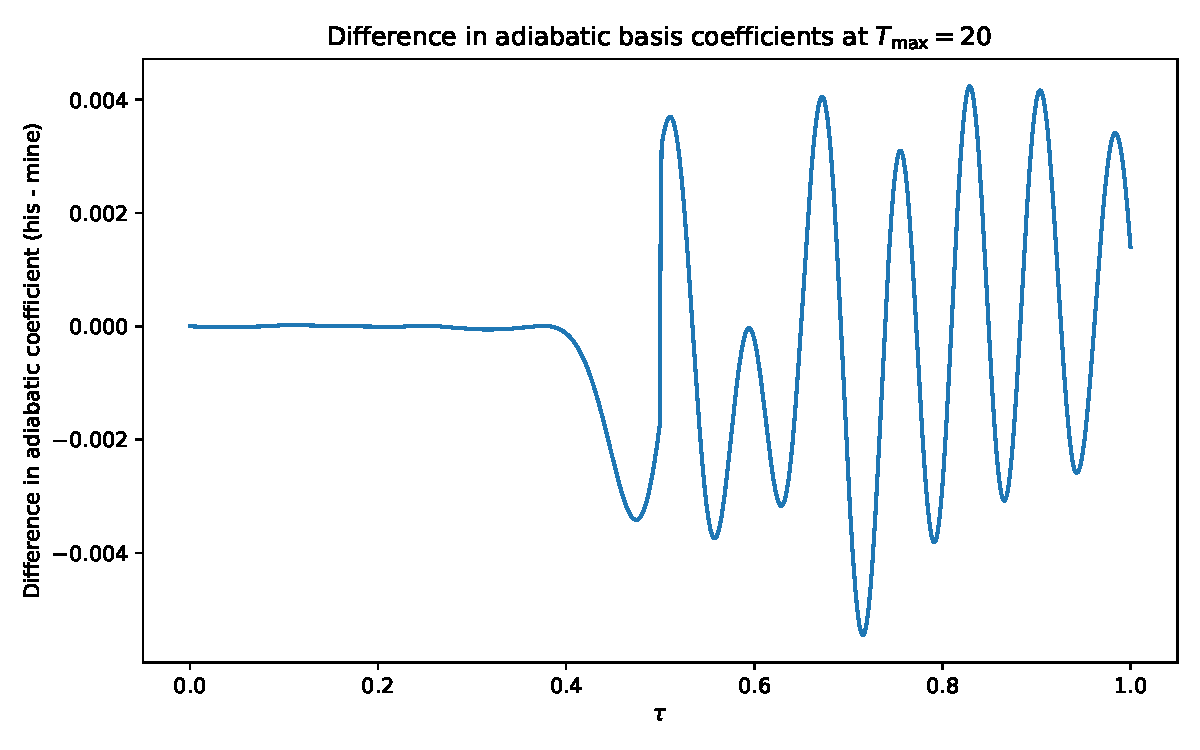
\includegraphics[width = \linewidth]{eivind_cut__trunc=10__eivind_diff_instantaneous_1.pdf}
    \caption{}
    \label{fig:2}
\end{figure}

\begin{figure}
    \centering
    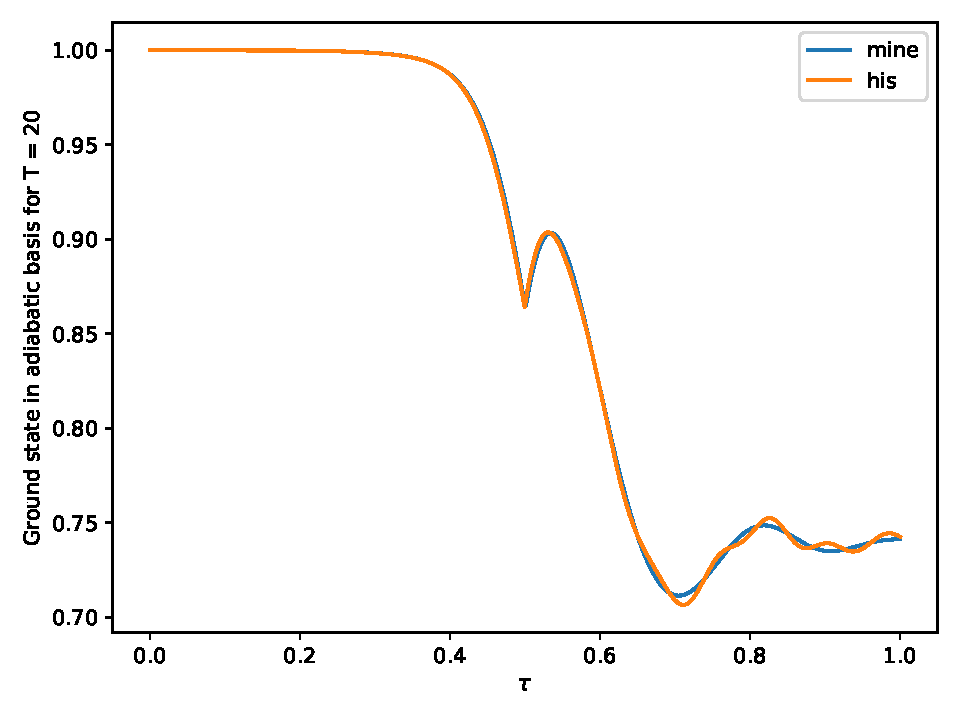
\includegraphics[width = \linewidth]{eivind_cut___eivind_instantaneous_basis.pdf}
    \caption{}
    \label{fig:3}
\end{figure}

\begin{figure}
    \centering
    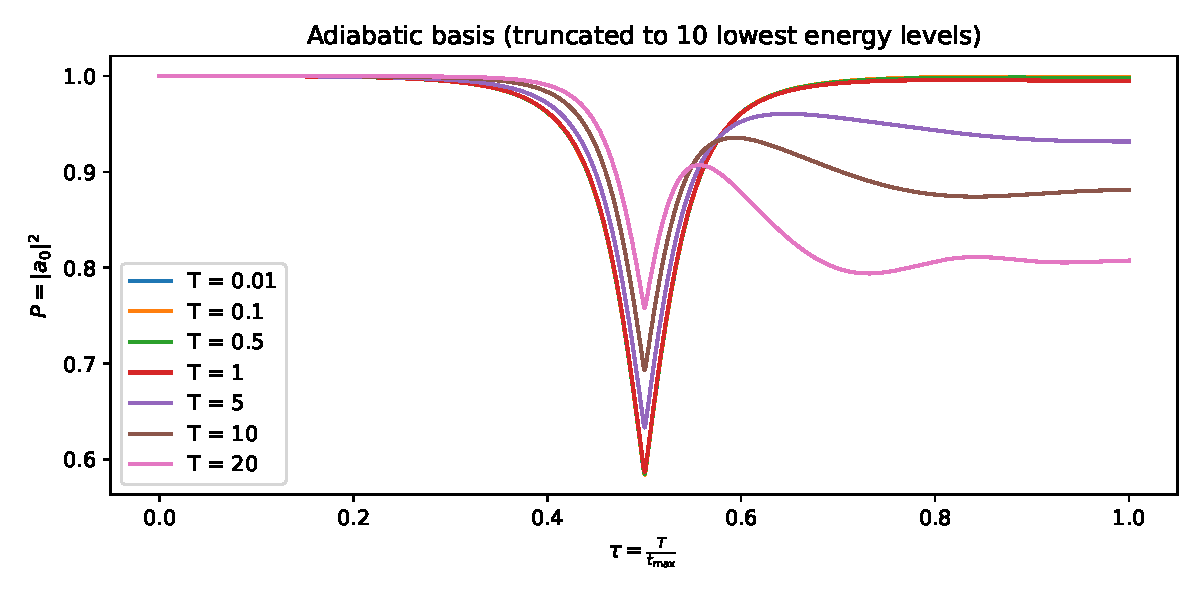
\includegraphics[width = \linewidth]{Proper_cut_chain_cut_chain_trunc=10_7_1.0_2.0_0.5_Adiabatic_precomputed_Kitaev_RK4_N=10_dt=0.001001001001001001_sparse.pdf}
    \caption{}
    \label{fig:4}
\end{figure}

\begin{figure}
    \centering
    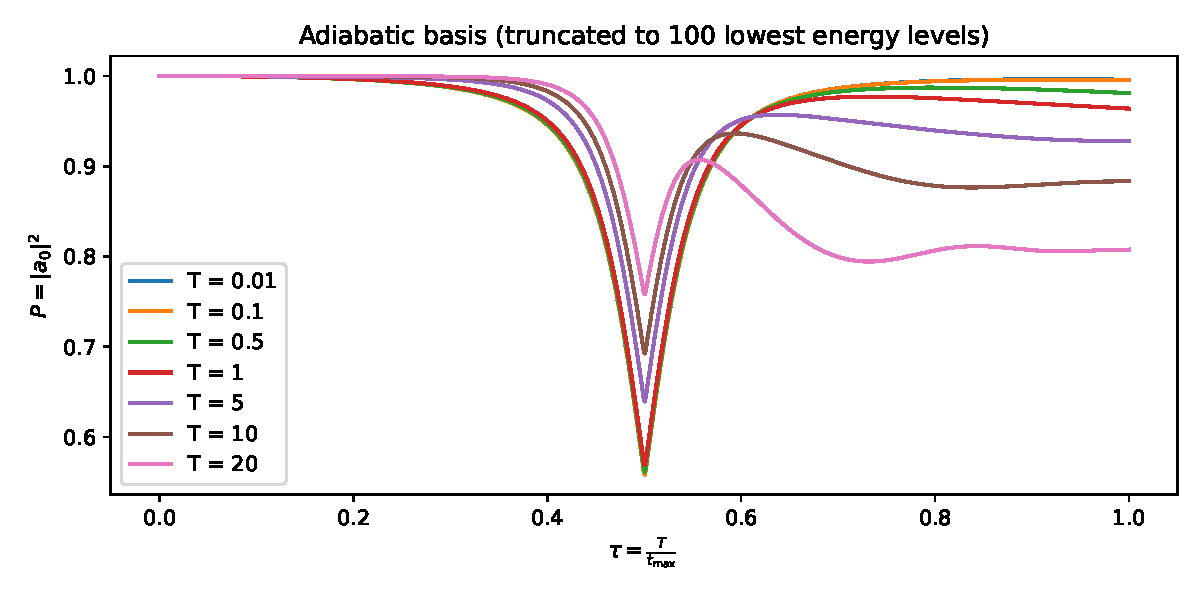
\includegraphics[width = \linewidth]{Proper_cut_chain_cut_chain_trunc=100_7_1.0_2.0_0.5_Adiabatic_precomputed_Kitaev_RK4_N=10_dt=0.001001001001001001_sparse.pdf}
    \caption{}
    \label{fig:5}
\end{figure}



\subsubsection{Schrodinger evolution vs adiabatic evolution}
Time and accuracy wrt truncation

\section{T-junction}
I need a supercomputer :/

\subsection{Pali X-gate}
Exchange 2 and 3

\subsection{Pauli Z-gate}
Exchange 1 and 2 (or 3 and 4)




\printbibliography

\appendix
\chapter{Calculations}
\section{Transforming Kitaev chain Hamiltonian to Majorana operators} 
\label{Appendix:Hamiltonian_Transformation}
This appendix shows how transform the original Kitaev chain Hamiltonian expressed in fermionic operators $a_j$ and $a_j^\dagger$ to being expressed in terms of the majorana operators $c_{2j-1}$ and $c_2j$. 

Starting with the majorana operators
\begin{align}
    c_{2j-1} &= e^{i \frac{\theta}{2}} a_j + e^{-i \frac{\theta}{2}}a_j^\dagger \\
    c_{2j} &= -ie^{i \frac{\theta}{2}} a_j + ie^{-i \frac{\theta}{2}}a_j^\dagger.
\end{align}
We can invert them, leading to four expressions
\begin{align}
    a_j &= e^{- i \frac{\theta}{2}} c_{2j-1} - e^{-i \theta} a_j^\dagger \\
    &= i e^{- i \frac{\theta}{2}} c_{2j} + e^{- i \theta} a_j^\dagger \\
    a_j^\dagger &= e^{i \frac{\theta}{2}} c_{2j-1} - e^{i\theta} a_j \\
    &= - i e^{i\frac{\theta}{2}} c_{2j} + e^{i \theta} a_j.
\end{align}
Combining the expressions for $a_j$, and for $a_j^\dagger$ we find
\begin{align}
    a_j &= \frac{1}{2} \left( e^{- i \frac{\theta}{2}} c_{2j-1} - e^{- i \theta} a_j^\dagger + e^{- i \theta} a_j^\dagger + i e^{- i \frac{\theta}{2}} c_2j \right) \\
    &= \frac{1}{2} e^{-i \frac{\theta}{2}} \left( c_{2j-1} + i c_{2j} \right)\\
    a_j^\dagger &= \frac{1}{2} \left( e^{i \frac{\theta}{2}} c_{2j-1} - e^{i\theta} a_j + e^{i \theta} a_j - i e^{i\frac{\theta}{2}} c_{2j}   \right) \\
    &= \frac{1}{2} e^{i \frac{\theta}{2}} \left( c_{2j-1} - i c_{2j}  \right).
\end{align}
We now substitute these expressions into the original Hamiltonian
\begin{align}
    H =& \sum_j\left[ - \omega \left(a_j^\dagger a_{j+1} + a_{j+1}^\dagger a_j  \right) - \mu \left(a_j^\dagger  a_j - \frac{1}{2} \right) + \Delta a_j a_{j+1} + \Delta^* a_{j+1}^\dagger a_j^\dagger \right]\\
    &= -\omega \sum_j  \frac{1}{2} e^{i \frac{\theta}{2}} \left( c_{2j-1} - i c_{2j}  \right) \frac{1}{2} e^{-i \frac{\theta}{2}} \left( c_{2(j+1)-1} + i c_{2(j+1)} \right) \\
    &-\omega \sum_j \frac{1}{2} e^{i \frac{\theta}{2}} \left( c_{2(j+1)-1} - i c_{2(j+1)}  \right) \frac{1}{2} e^{-i \frac{\theta}{2}} \left( c_{2j-1} + i c_{2j} \right)\\
    &- \mu \sum_j \left(\frac{1}{2} e^{i \frac{\theta}{2}} \left( c_{2j-1} - i c_{2j}  \right) \frac{1}{2} e^{-i \frac{\theta}{2}} \left( c_{2j-1} + i c_{2j} \right)  - \frac{1}{2}\right) \\
    &+ \Delta \sum_j \frac{1}{2} e^{-i \frac{\theta}{2}} \left( c_{2j-1} + i c_{2j} \right) \frac{1}{2} e^{-i \frac{\theta}{2}} \left( c_{2(j+1)-1} + i c_{2(j+1)} \right) \\
    &+ \Delta^* \sum_j \frac{1}{2} e^{i \frac{\theta}{2}} \left( c_{2(j+1)-1} - i c_{2(j+1)}  \right) \frac{1}{2} e^{i \frac{\theta}{2}} \left( c_{2j-1} - i c_{2j}  \right)\\
    &= - \frac{\omega}{4} \sum_j \left( c_{2j-1} c_{2j + 1} + i c_{2j-1} c_{2j + 2} - i c_{2j} c_{2j + 1} + c_{2j} c_{2j + 2} \right) \\
    &- \frac{\omega}{4} \sum_j \left( c_{2j+1} c_{2j - 1} + i c_{2j + 1} c_{2j} - i c_{2j + 2} c_{2j - 1} + c_{2j + 2} c_{2j}\right)\\
    & -\frac{\mu}{4} \sum_j \left( c_{2j-1}^2 + ic_{2j-1} c_{2j} - i c_{2j} c_{2j-1} + c_{2j}^2 - 2 \right) \\
    &+ \frac{|\Delta|}{4}e^{i\theta} \sum_j e^{-i \theta} \left( c_{2j-1} c_{2j+1} + i c_{2j-1} c_{2j+2} + i c_{2j} c_{2j+1} - c_{2j} c_{2j+2} \right) \\
    &+ \frac{|\Delta|}{4} e^{-i\theta} \sum_j e^{i\theta}\left( c_{2j+1} c_{2j-1} - i c_{2j + 1} c_{2j} - i c_{2j+2} c_{2j-1} - c_{2j+2} c_{2j}\right) \\
    &= - \frac{\omega}{4} \sum_j \left( 0 + 2 i c_{2j-1} c_{2j+2} - 2i c_{2j}c_{2j+1} + 0\right) \\
    &- \frac{\mu}{4} \sum_j \left( 2i c_{2j-1}c_{2j} + 2 - 2\right)\\
    &+ \frac{|\Delta|}{4}\sum_j \left( 0 + 2i c_{2j-1}c_{2j+2} + 2i c_{2j} c_{2j+1} + 0  \right) \\
    &= \frac{i}{2} \sum_j \left[-\mu c_{2j-1} c_{2j} + \left(\omega + \left|\Delta \right|  \right) c_{2j} c_{2j+1} + \left(-\omega + \left| \Delta \right| \right) c_{2j-1} c_{2j+2} \right]
\end{align}
Where we used $\Delta = |\Delta|e^{i\theta}$ and the anticommutation relations
\begin{align}
    \left\{ c_l, c_m \right\} &= c_l c_m + c_m c_l = 2\delta_{lm} \\
    c_l c_m &= - c_m c_l (m \neq l)\\
    c_l^2 &= 1.
\end{align}


\end{document}
